\documentclass[journal]{IEEEtran}
\ifCLASSINFOpdf
\else
\fi
\hyphenation{op-tical net-works semi-conduc-tor}
\usepackage{booktabs}
\usepackage{float}
\usepackage{graphicx}
\usepackage{amsmath} 

\begin{document}
\title{Amplificadores basados en FET y circuitos de conmutación}
\author{Guido P. Krisdel Pamela, Gamboa Q. María José} 
\markboth{ITCR. Escuela de Ingeniería Electrónica. Laboratorio 8 – Amplificadores basados en JFET y circuitos de conmutación}
{Shell \MakeLowercase{\textit{et al.}}: Bare Demo of IEEEtran.cls for IEEE Journals}

\maketitle
\renewcommand{\abstractname}{Resumen}
\begin{abstract}
En este informe se estudia el comportamiento de amplificadores con transistores JFET, específicamente en configuraciones de fuente común y drenador común. Se construyeron y analizaron ambos circuitos, evaluando sus parámetros en corriente continua (DC) y corriente alterna (CA), incluyendo ganancia de tensión, desfase entre señales de entrada y salida, y la respuesta ante fallas comunes. Además, se observó el efecto de la variación en la resistencia de carga y el uso de una fuente de corriente en la mejora de la ganancia del amplificador. Los resultados permiten comprender el funcionamiento, limitaciones y ventajas de estas configuraciones en aplicaciones electrónicas donde se requiere amplificación de señales pequeñas.
\end{abstract}

\renewcommand{\IEEEkeywordsname}{Palabras clave}
\begin{IEEEkeywords}
amplificador JFET, fuente común, drenador común, ganancia de tensión
\end{IEEEkeywords}

\IEEEpeerreviewmaketitle

\section{Introduction}
\IEEEPARstart{L}{os}
amplificadores utilizando transistores JFET son fundamentales en el diseño de circuitos electrónicos debido a su alta impedancia de entrada y bajo consumo de potencia. Entre las configuraciones más comunes se encuentran el amplificador en fuente común y el amplificador en drenador común, cada uno con características particulares que afectan el comportamiento de la señal amplificada.
\par El objetivo principal del experimento fue analizar el comportamiento de estas configuraciones ante distintas condiciones de operación, midiendo parámetros tanto en corriente continua como en corriente alterna. Se estudió la respuesta del circuito ante cambios en la resistencia de carga, así como los efectos de polarización mediante una fuente de corriente. Además, se evaluó la ganancia de tensión, la diferencia de fase entre la señal de entrada y salida, y la respuesta del circuito ante fallas específicas.
\par A partir del análisis experimental, se concluye que la elección de la configuración y polarización del JFET influye directamente en el rendimiento del amplificador. Esta comprensión es esencial para el diseño de sistemas que requieren amplificación precisa y eficiente de señales en aplicaciones electrónicas variadas.

\section{MATERIALES Y EQUIPO}
Para la realización de ambas configuraciones del experimento se emplearon los siguientes equipos de medición:
\begin{itemize}
    \item 1 Generador de señales
    \item 1 Osciloscopio
    \item 1 Multímetro
\end{itemize}
\par Para la configuración del amplificador en fuente común se empleó los siguientes componentes electrónicos:
\begin{itemize}
    \item 1 Resistencia de 56 $\Omega$
    \item 1 Resistencia de 6.8k $\Omega$
    \item 1 Resistencia de 10k $\Omega$
    \item 1 Resistencia de 100k $\Omega$
    \item 1 Resistencia de 10M $\Omega$
    \item 1 Capacitor de 0.1$\mu$ F
    \item 1 Capacitor de 1$\mu$ F
    \item 1 Capacitor de 10$\mu$ F
    \item 1 Transistor JFET 2N5458 
\end{itemize}
\par Para la configuración del amplificador en drenador común se empleó los siguientes componentes electrónicos:
\begin{itemize}
    \item 1 Resistencia de 100 $\Omega$
    \item 1 Resistencia de 1k $\Omega$
    \item 1 Resistencia de 10k $\Omega$
    \item 1 Resistencia de 100k $\Omega$
    \item 1 Resistencia de 220 $\Omega$
    \item 1 Resistencia de 1M $\Omega$
    \item 1 Capacitor de 0.1$\mu$ F
    \item 1 Capacitor de 10$\mu$ F
    \item 1 Potenciómetro de 500 $\Omega$
    \item 2 Transistores JFET 2N5458
\end{itemize}

\section{Resultados Experimentales}
\par Se presentan los datos obtenidos durante la ejecución del experimento en la parte correspondiente al amplificador con drenador común. Se incluyen mediciones realizadas con los instrumentos de laboratorio, así como observaciones relevantes sobre el comportamiento del circuito. Además, se comparan los resultados experimentales con los valores teóricos y simulaciones para analizar la precisión de las mediciones.
\par Para garantizar la precisión de los resultados obtenidos en el experimento, se realizó una medición previa de los valores de las resistencias y capacitores, y así, asegurar que los valores reales estuvieran dentro de la tolerancia especifica. Los valores obtenidos en la medición se presentan en la siguiente tabla:
\begin{table}[h]
    \caption{Comparación entre valores teóricos y experimentales de resistencias.}
    \centering
    \renewcommand{\arraystretch}{1.2} % Ajusta la altura de las filas
    \begin{tabular}{|l|p{2cm}|p{2cm}|p{2cm}|}
        \hline
        & \textbf{Valor Teórico [$\Omega$]} & \textbf{Valor Experimental [$\Omega$]} & \textbf{Porcentaje de error [\%]} \\
        \hline
        R1 & 100  & 101.003  & 1 \\
        \hline
        R2 & 1k   & 0.997k  & 0.30 \\
        \hline
        R3 & 10k & 9.909k & 0.91 \\
        \hline
        R3 & 220 & 220.672 & 0.30 \\
        \hline
        R3 & 1M & 0.986M & 1.4 \\
        \hline
    \end{tabular}
    \label{tab:resistencias}
\end{table}
\par A partir de los datos obtenidos, se evidencia que los valores experimentales de las resistencias presentan una buena concordancia con los valores teóricos. El porcentaje de error registrado en cada caso se mantiene igual o por debajo de 1.4, lo cual es coherente con las tolerancias esperadas en componentes electrónicos de uso general. Estos resultados permiten asegurar que los componentes empleados son adecuados para el desarrollo experimental y garantizan mediciones confiables.
\par Se procedió con la construcción del circuito amplificador en drenador común, según lo ilustrado en la Figura 1. 
\begin{figure}[H]
    \centering
    \includegraphics[width=0.5\textwidth]{Media/amplificador_drenador_común.png}
    \caption{Amplificador en drenador común.}
    \label{fig:amplificador_drenador_común.}
\end{figure}
\par Una vez ensamblado el circuito, se midieron las tensiones en corriente directa (CD) en los terminales de drenador, fuente y compuerta del transistor JFET. A partir de la tensión medida en la resistencia \( R_S \), se calculó la corriente \( I_D \) correspondiente. Todos los valores obtenidos fueron registrados en la Tabla 2 para su análisis comparativo.
\begin{table}[h]
    \caption{Comparación parámetros CD para el amplificador en drenador común}
    \centering
    \renewcommand{\arraystretch}{1.2} % Ajusta la altura de las filas
    \begin{tabular}{|l|p{2cm}|p{2cm}|p{2cm}|}
        \hline
        & \textbf{Valor Teórico} & \textbf{Valor Experimental} & \textbf{Porcentaje de error [\%]} \\
        \hline
        \( V_G \) & 0 V  & 0.054m V  & 0.05 \\
        \hline
        \( V_S \) & 209.402m V   & 210.121m V  & 0.34 \\
        \hline
        \( V_D \) & 15 V & 15.011 V & 0.07 \\
        \hline
        \( I_D \) & 269, 847m A & 268.672m A & 0.43 \\
        \hline
    \end{tabular}
    \label{tab:resistencias}
\end{table}
\par En la comparación de los parámetros del amplificador en drenador común, se observa que los valores experimentales obtenidos están muy cerca de los valores teóricos, lo que indica una buena concordancia entre ambos. El porcentaje de error se mantiene bajo en todos los casos, con el valor más bajo registrado en \( V_G \), y el más alto en \( I_D \). En general, los errores porcentuales son mínimos, lo que refleja una correcta implementación del amplificador en drenador común.
\par Posteriormente, se utilizaron las puntas del osciloscopio para observar simultáneamente la señal de entrada y la señal de salida en corriente alterna (CA), con el fin de analizar su comportamiento dinámico, según lo ilustrado en la Figura 2. 
\begin{figure}[H]
    \centering
    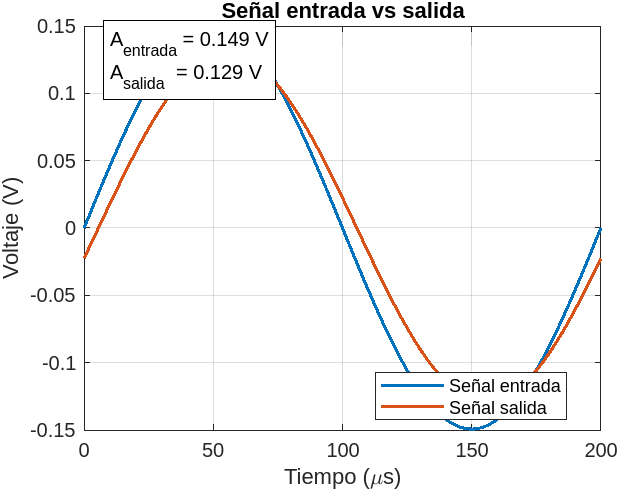
\includegraphics[width=0.5\textwidth]{Media/onda_entrada_salida.png}
    \caption{Onda entrada vs salida .}
    \label{fig:onda_entrada_salida.}
\end{figure}
\par Se determinó el desfase entre ambas señales y se calculó la ganancia de tensión del amplificador. Todos los valores obtenidos fueron registrados en la Tabla 3 para su análisis comparativo.
\begin{table}[h]
    \caption{Comparación parámetros CA para el amplificador en drenador común}
    \centering
    \renewcommand{\arraystretch}{1.2} % Ajusta la altura de las filas
    \begin{tabular}{|l|p{2cm}|p{2cm}|p{2cm}|}
        \hline
        & \textbf{Valor Teórico} & \textbf{Valor Experimental} & \textbf{Porcentaje de error [\%]} \\
        \hline
        \( V_{ent}\) & 149.268m V   & 150m V  & 0.49 \\
        \hline
        \( V_{SAL} \) & 129.198m V    & 126m V  & 2.47 \\
        \hline
        \( A_V \) & 0.865 & 0.840 & 2.89 \\
        \hline
        Desfase & $0^\circ$ & $0^\circ$ & 0 \\
        \hline
    \end{tabular}
    \label{tab:resistencias}
\end{table}
\par En la comparación de los parámetros de corriente alterna (CA) para el amplificador en drenador común, se observa que los valores experimentales están en cercanía con los valores teóricos. El porcentaje de error es bajo en general, destacando el valor de \( V_{ent}\) con un error de 0.49, mientras que el valor más alto corresponde a \( V_{SAL} \) con un error de 2.47. El factor de amplificación \( A_V \) presenta un error de 2.89, lo que es también un valor relativamente bajo. Además, el desfase entre las señales es nulo, coincidiendo con el valor teórico de $0^\circ$. Estos resultados indican que el comportamiento del amplificador en drenador común es consistente con las expectativas teóricas en cuanto a su desempeño en corriente alterna.
\par Seguidamente, se aumentó progresivamente la amplitud de la señal de entrada\( V_S \) con el fin de observar el comportamiento del amplificador ante señales de mayor exigencia. Se encontró que con una amplitud de 255m\( V_P \), la salida se mantenía sin distorsión visible. No obstante, a partir de 265m\( V_P \) comenzaron a notarse ligeras alteraciones en la forma de onda, que se hicieron más evidentes en 270m\( V_P \), y finalmente se observó un recorte claro en 300m\( V_P \). 
\par En ese punto, la señal de salida alcanzó un valor máximo de 262.6913m\( V_P \) y un valor mínimo de -190.835m\( V_P \), evidenciando que el amplificador dejó de operar dentro de su región lineal. Este comportamiento se debe a que el transistor JFET alcanza sus límites de conducción: al aumentar demasiado la amplitud de la señal de entrada, el transistor entra en saturación o corte, impidiendo que la señal de salida reproduzca fielmente la forma de la señal de entrada.




\begin{figure}[H]
    \centering
    \includegraphics[width=0.5\textwidth]{Media/diagrama_flujo_restador.png}
    \caption{Diagrama de flujo del funcionamiento del Restador parametrizable.}
    \label{fig:diagrama_flujo_restador}
\end{figure}

\par .........................
\par ..................


\begin{figure}[H]
    \centering
    \includegraphics[width=0.5\textwidth]{Media/diagrama_flujo_restador.png}
    \caption{Diagrama de flujo del funcionamiento del Restador parametrizable.}
    \label{fig:diagrama_flujo_restador}
\end{figure}

\begin{figure}[H]
    \centering
    \includegraphics[width=0.5\textwidth]{Media/diagrama_flujo_restador.png}
    \caption{Diagrama de flujo del funcionamiento del Restador parametrizable.}
    \label{fig:diagrama_flujo_restador}
\end{figure}

\par ................ 

\begin{figure}[H]
    \centering
    \includegraphics[width=0.5\textwidth]{Media/diagrama_flujo_restador.png}
    \caption{Diagrama de flujo del funcionamiento del Restador parametrizable.}
    \label{fig:diagrama_flujo_restador}
\end{figure}
\begin{figure}[H]
    \centering
    \includegraphics[width=0.5\textwidth]{Media/diagrama_flujo_restador.png}
    \caption{Diagrama de flujo del funcionamiento del Restador parametrizable.}
    \label{fig:diagrama_flujo_restador}
\end{figure}
\par .................................
\par ........
\begin{figure}[H]
    \centering
    \includegraphics[width=0.5\textwidth]{Media/diagrama_flujo_restador.png}
    \caption{Diagrama de flujo del funcionamiento del Restador parametrizable.}
    \label{fig:diagrama_flujo_restador}
\end{figure}
\par ...................................
\begin{table}[h]
\caption{Comparación entre valores teóricos y experimentales de voltajes.}
    \centering
    \renewcommand{\arraystretch}{1.2} % Ajusta la altura de las filas
    \begin{tabular}{|l|p{2cm}|p{2cm}|p{2cm}|}
        \hline
        & \textbf{Valor Teórico [V]} & \textbf{Valor Experimental [V]} & \textbf{Porcentaje de error [\%]} \\
        \hline
        D1 & 0.7  & 0.698  & 0.28 \\
        \hline
    \end{tabular}
    \label{tab:voltajes}
\end{table}

\par ..................................
\begin{figure}[H]
    \centering
    \includegraphics[width=0.5\textwidth]{Media/diagrama_flujo_restador.png}
    \caption{Diagrama de flujo del funcionamiento del Restador parametrizable.}
    \label{fig:diagrama_flujo_restador}
\end{figure}
\begin{figure}[H]
    \centering
    \includegraphics[width=0.5\textwidth]{Media/diagrama_flujo_restador.png}
    \caption{Diagrama de flujo del funcionamiento del Restador parametrizable.}
    \label{fig:diagrama_flujo_restador}
\end{figure}

\par .............................
\par .............................. 
\begin{figure}[H]
    \centering
    \includegraphics[width=0.5\textwidth]{Media/diagrama_flujo_restador.png}
    \caption{Diagrama de flujo del funcionamiento del Restador parametrizable.}
    \label{fig:diagrama_flujo_restador}
\end{figure}
\begin{figure}[H]
    \centering
    \includegraphics[width=0.5\textwidth]{Media/diagrama_flujo_restador.png}
    \caption{Diagrama de flujo del funcionamiento del Restador parametrizable.}
    \label{fig:diagrama_flujo_restador}
\end{figure}

\par ...........................
\par ...................................
\begin{figure}[H]
    \centering
    \includegraphics[width=0.5\textwidth]{Media/diagrama_flujo_restador.png}
    \caption{Diagrama de flujo del funcionamiento del Restador parametrizable.}
    \label{fig:diagrama_flujo_restador}
\end{figure}
\begin{figure}[H]
    \centering
    \includegraphics[width=0.5\textwidth]{Media/diagrama_flujo_restador.png}
    \caption{Diagrama de flujo del funcionamiento del Restador parametrizable.}
    \label{fig:diagrama_flujo_restador}
\end{figure}
\par ......................
\par .....................................

\begin{equation*}
    V_{R2}=2.921
\end{equation*}

\par ......................

\begin{table}[h]
\caption{Valor resistencia de carga modificada.}
    \centering
    \renewcommand{\arraystretch}{1.2} % Ajusta la altura de las filas
    \begin{tabular}{|l|p{2cm}|p{2cm}|p{2cm}|}
        \hline
        & \textbf{Valor Teórico [k$\Omega$]} & \textbf{Valor Experimental [k$\Omega$]} & \textbf{Porcentaje de error [\%]} \\
        \hline
        RL & 10  & 9.892  & 1.08 \\
        \hline
    \end{tabular}
    
    \label{tab:resistencia_carga}
\end{table}
\par ..........................
\par .............................

\begin{figure}[H]
    \centering
    \includegraphics[width=0.5\textwidth]{Media/diagrama_flujo_restador.png}
    \caption{Diagrama de flujo del funcionamiento del Restador parametrizable.}
    \label{fig:diagrama_flujo_restador}
\end{figure}
\begin{figure}[H]
    \centering
    \includegraphics[width=0.5\textwidth]{Media/diagrama_flujo_restador.png}
    \caption{Diagrama de flujo del funcionamiento del Restador parametrizable.}
    \label{fig:diagrama_flujo_restador}
\end{figure}
\begin{figure}[H]
    \centering
    \includegraphics[width=0.5\textwidth]{Media/diagrama_flujo_restador.png}
    \caption{Diagrama de flujo del funcionamiento del Restador parametrizable.}
    \label{fig:diagrama_flujo_restador}
\end{figure}
\begin{figure}[H]
    \centering
    \includegraphics[width=0.5\textwidth]{Media/diagrama_flujo_restador.png}
    \caption{Diagrama de flujo del funcionamiento del Restador parametrizable.}
    \label{fig:diagrama_flujo_restador}
\end{figure}

\par .........................
\par ........................


\section{Conclusion}
\par ....................................
\par ........................
\par .........................

\appendices
\section{}
\noindent\textbf{Análisis del Divisor de Tensión}
\par En los circuitos analizados, las resistencias R2 y RL conforman un divisor de tensión que influye en la señal de salida [1]. Aplicando la ecuación del divisor de tensión:
\begin{equation}
    V_{out}=(V_{in}\times R_L)/(R_2+\ R_L\ )
\end{equation}
\par Se puede calcular la tensión que se observa en la salida en función de los valores de las resistencias. En particular, la reducción de RL afecta directamente la caída de tensión y modifica la amplitud de la señal de salida [1].
\\
\newline
\textbf{Deducción del Recorte de Señal por el Diodo}
\par El diodo 1N914, cuando se encuentra en polarización directa, permite el paso de corriente y presenta una caída de tensión aproximada de 0.7V [1]. Cuando la señal de entrada cae por debajo de este umbral, el diodo se bloquea y evita el paso de corriente, recortando la señal en dicho punto [2]. Este fenómeno es clave en circuitos recortadores, donde la forma de la señal de salida es modificada significativamente por la presencia del diodo. La ecuación de la señal recortada puede expresarse como:
\begin{equation}
    V_{OUT}=V_{IN}-V_{D}\ \ cuando\ V_{IN}>V_{D}
\end{equation}
\par Lo que confirma que la amplitud máxima de la señal de salida se ve limitada por el umbral del diodo [1].
\\
\newline
\textbf{Frecuencia y Período de la Señal}
\par La frecuencia y el período son parámetros fundamentales en el análisis de señales sinusoidales como las utilizadas en este experimento [1]. La relación entre ambas magnitudes se expresa mediante la ecuación:
\begin{equation}
    T=1/f
\end{equation}
Donde:
\begin{itemize}
    \item T es el período de la señal en segundos [s]
	\item  f es la frecuencia de la señal en Hertz [Hz]
\end{itemize}
\\
\newline
\par En este experimento, la señal generada tiene una frecuencia de 1kHz, lo que implica un período de:
\begin{equation}
    T=1/1000=1ms
\end{equation}
\par Esto significa que la onda completa se repite cada 1 milisegundo. 
\\
\newline
\textbf{Cálculo de la Tensión en R2 mediante la Ley de Kirchhoff}
\par Dada la onda de tensión sobre la carga y la fuente en el circuito de la Figura 6, se puede utilizar la Ley de Tensiones de Kirchhoff para obtener la tensión sobre la resistencia R2 [1]. En el circuito, las tensiones relevantes en el lazo donde está la resistencia R2 son:
\begin{itemize}
	\item V$_S$: Voltaje de la fuente de señal
	\item V$_{R2}$: Voltaje en la resistencia R2
	\item V$_Y$: Voltaje en el nodo de salida del circuito
\end{itemize}
\\
\newline
Aplicando la Ley de Kirchhoff:
\begin{equation}
    V_{R2}=V_S-V_Y
\end{equation}
Dado que:
\begin{equation}
    V_Y=V_{D1}-V_{RL}
\end{equation}
Se expresa la ecuación como:
\begin{equation}
    V_{R2}=V_S-(V_{D1}-V_{RL}\ )
\end{equation}
Sustituyendo los valores:
\begin{equation}
    V_{R2}=3V \ (0.7V-621.502mV\ )=2.921V
\end{equation}


\ifCLASSOPTIONcaptionsoff
  \newpage
\fi

\begin{thebibliography}{1}

\bibitem{IEEEhowto:kopka}
H.~Kopka and P.~W. Daly, \emph{A Guide to \LaTeX}, 3rd~ed.\hskip 1em plus
  0.5em minus 0.4em\relax Harlow, England: Addison-Wesley, 1999.

\end{thebibliography}

\begin{IEEEbiography}{Michael Shell}
Biography text here.
\end{IEEEbiography}

\begin{IEEEbiographynophoto}{John Doe}
Biography text here.
\end{IEEEbiographynophoto}

\begin{IEEEbiographynophoto}{Jane Doe}
Biography text here.
\end{IEEEbiographynophoto}

\end{document}
